\documentclass[a4paper,oneside]{memoir}
\usepackage[T1]{fontenc}
\usepackage[utf8]{inputenc}
\usepackage[english]{babel}


\usepackage[format=hang]{caption,subfig}
\usepackage{graphicx}
\usepackage{pdflscape} % Gør landscape-environmentet tilgængeligt
\usepackage[draft]{fixme}     % Indsæt "fixme" noter i drafts.
\usepackage{hyperref}  % Indsæter links (interne og eksterne) i PDF


%% \renewcommand{\ttdefault}{pcr} % Bedre typewriter font
%% %\usepackage[sc]{mathpazo}     % Palatino font
%% \renewcommand{\rmdefault}{ugm} % Garamond
\usepackage[garamond]{mathdesign}

%\overfullrule=5pt
%\setsecnumdepth{part}
\setcounter{secnumdepth}{-1} % Sæt overskriftsnummereringsdybde. Disable = -1.

\newcommand{\EDSL}{EDSL (Embedded Domain Specific Language) \renewcommand{\EDSL}{ EDSL }}
\hyphenation{da-ta-be-hand-ling}
\hyphenation{pro-gram-me-rings-sprog-et}
\hyphenation{brug-es}

\title{Synopsis}

\author{%Johan Brinch (zerrez@gmail.com) \and
Morten Brøns-Pedersen (mortenbp@gmail.com) \and
Jesper Reenberg (jesper.reenberg@gmail.com)}


\date{\today}
\pagestyle{plain}


\begin{document}
\maketitle

\section{Project title}

``Skal vi lege Dr.?''
\fixme{Proper title: SMLserver?}

\section{Project overview}

Programs written in functional programming languages has a wide variety of
advantages that make them specially suited for quick and correct statical
analysis.

\fixme{hvilke?}

The main goal of this project is to exploit this statical analysis to
perform semi automatic refactoring of function definitions to standard
forms. That is, given some predefined transformations of functions, to
hint the programmer of possible rewritings that will improve the code
she is working on. These hints should prove helpful in writing idiomatic
functional code.

\fixme{bør andre typer plugins nævnes? Disse kan jo evt blot pilles væk i
  afgrænsningen}


%\begin{quotation}
%  Programmer i deklarative programmeringssprog har en række fordele,
%  som gør dem særdeles velegnet til hurtig og korrekt statisk
%  analyse.
%
%  Formålet med denne opgave er at udnytte ovenstående til at foretage
%  halvautomatiske refaktoreringer, som kun vanskeligt kan benyttes (eller
%  sjældent er relevante) i øvrige sprog.
%\end{quotation}

\section{Elaboration}

\subsection{Introduction}

The target audience for this tool is novice programmers in functional
programming languages who is not used to work with the programming patterns
and -templates from this paradigme.

% \begin{quotation}
%   Målgruppen for det udviklede værktøj er novicer i
%   funktionsprogrammering, som ikke er vant til at benytte de særlige
%   programmeringsmønstre og -skabeloner fra dette paradigme.
% \end{quotation}


\subsection{Project Overview}
\fixme{should implementation details be included?.. Yes in abstract terms.}

We focus on creating a software package that will be easy to extend in
the future. The software consists of two parts; an extension for Emacs
that is responsible for doing all communication with the programmer,
and a backend that implement the actual code-specific functionality.

The backend part is split into a few major parts:
\begin{description}
\item[Project manager.] The backend should be able to work on whole
  projects. The project manager is required to handle parsing of ML
  Basis files (.mlb). The project manager can later be extended to
  actually manage projects. That is supply means for adding and
  removing files and for updating ML Basis files with such new
  information.
\item[Parser.] Virtually every software system that does some analysis
  on source code needs the source code to be represented as a syntax
  tree. The parser handles the task of creating syntax trees from
  source files. The least amount of work to be done is to create
  concrete syntax trees that exactly describe the source text. This
  can later be extended with further analysis to obtain type
  information, remove derived forms etc.
\item[Plugins.] When the source text has been preprocessed the actual
  plugins can work on its syntax tree. The plugins provides
  information that will be presented to the user through the Emacs
  GUI. This is where the refactoring suggestions will be generated.
\end{description}

Apart from the above the parts need to be tied together and
communication with the user taken care of.
\fixme{communication has been taken care of by Emacs extension?}

\subsubsection{Data flow}
\fixme{discuss the dataflow:}
\fixme{Datastrukturer i flow ned igennem, skal bygge videre og ikke smide noget
  data væk.}

\subsubsection{Project Manager}

\subsubsection{Source Management}


The \texttt{Source Management} component is responsible for the actual
IO handling when some component (e.g., the \texttt{SML Parser}) wants
to know the actual contents of a file. This way it can implement a
caching method of own choosing, to speed up content retrieval.


\subsubsection{SML Parser}
\begin{itemize}
\item support for MosML \texttt{load}

\item Should run in a thread for it self, so it can be restarted if
  the file being analyzed changes
\end{itemize}

\subsubsection{Plugins}

\fixme{elaborate about the refactoring plugin}
\fixme{Plugins skal kompiles med. (Alle plugins skal være slukket fra start)}

\subsubsection{IO Communication Bridge}

\fixme{detailed explanation of the communication possibilities, without the
  actual protocol (json)}


\section{Learning objectives}

\begin{enumerate}
\item To develop structured, flexible and well-documented software for
  manipulation of source code.
\item To understand and describe a formal mathematical transformation
  and develop software to perform such.
\end{enumerate}


\section{Task's}

\begin{enumerate}
\item Design the \texttt{Source Management} API. (1 week)

\item Implement a \textit{.MLB}-file parser (\texttt{MLB Parser}) from the MLB
  definition (1 week)
\url{http://www.itu.dk/research/mlkit/index.php/ML_Basis_Files}

\item Design the concrete syntax tree to be used by the \texttt{SML
    Parser}. This needs to be done correct the first time. (1 week)

\item Create the \texttt{SML Parser} (3 weeks).

\item Create the \texttt{Refactoring Plugin} (3 weeks).

\item Create the \texttt{SMLserver} (1 week).
  \begin{itemize}
  \item Connect the \texttt{SML Parser} and \texttt{Refactoring
      Plugin} using threads
  \end{itemize}

\item Create the missing links in the \texttt{SMLserver} (2 weeks)
  \begin{itemize}
  \item Create the \texttt{non project files parser}\footnote{correct to the
      right name} and connect it with the \texttt{MLB Parser} into the
    \texttt{Source Management}.

  \item Create the \texttt{Project Manager}.

  \item Connect the \texttt{Source Management} with the \texttt{Project
      Manager}.

  \item Connect the \texttt{Project Manager} with the \texttt{SML Parser}.
  \end{itemize}

\item Create the \texttt{Communication Interface} between the
  \texttt{SMLserver} and the front end
  \begin{itemize}
  \item Create a plugin to the front end that will support the
    \texttt{Communication Interface}.
  \end{itemize}
\end{enumerate}


\section{Limitations}

\begin{enumerate}
\item There will not be developed a \textit{.CM}-file parser to the
  \texttt{Source Description} interface.

\item The \texttt{SML Parser} will not handle syntax errors.

\item The \texttt{Source Management}

  \begin{itemize}
  \item will not implement caching, but just read data from disk when
    requested.

  \item will not implement the patch system.
  \end{itemize}

\item No user documentation of software will be produced (e.g.,
  manual, user guide)
\end{enumerate}


\section{Expansion (``nice to have'')}


\begin{enumerate}

\item An incremental \texttt{SML Parser}

\item That the \texttt{SML Parser} can handle syntax errors. That is,
  by skipping the source code until next valid expression and then
  continue to parse. The skipped part could be reported to the
  front-end and then handled appropriately (e.g., underlined).

\item The \texttt{Source Management} implements a patch system, so
  when a component request the content of a file, which is is edited
  in the IDE and not saved to the file system, it gets the content
  from the file system but where a line is edited in the editor it
  gets the line from the editor instead.


\item Support of \texttt{DocString} by the \texttt{Communication
    Bridge} so when the front end hovers a function call it can show
  the \texttt{DocString} describing parameters and what the function
  does.

\item Der kan tænkes flere forskellige SML parser niveauer
  \begin{itemize}

  \item Der skal derfor indføres "runlevels". Så ved hvert parsnings
    afslut skal de plugin spawnes som "hooker" dette parsetræ
    (evt. kun 1 tråd der efter tur eksekverer alle plugins som hooker
    den givne level), samtidig med at der spawnes en tråd til at lave
    næste parsnings niveau.
  \end{itemize}


\item The \texttt{Source Managemnt} needs to implement some sort of patch
  system, such that when a component request the content of a file and the user
  has made changes in the IDE that is not save to the file, these changes are
  also reflected in the content returned to the component.

\end{enumerate}


\appendix

\chapter{Timetable}

\fixme{her kommer en tidstabel}

\chapter{Flow diagram}
\fixme{Make diagram bigger and still fit on page}
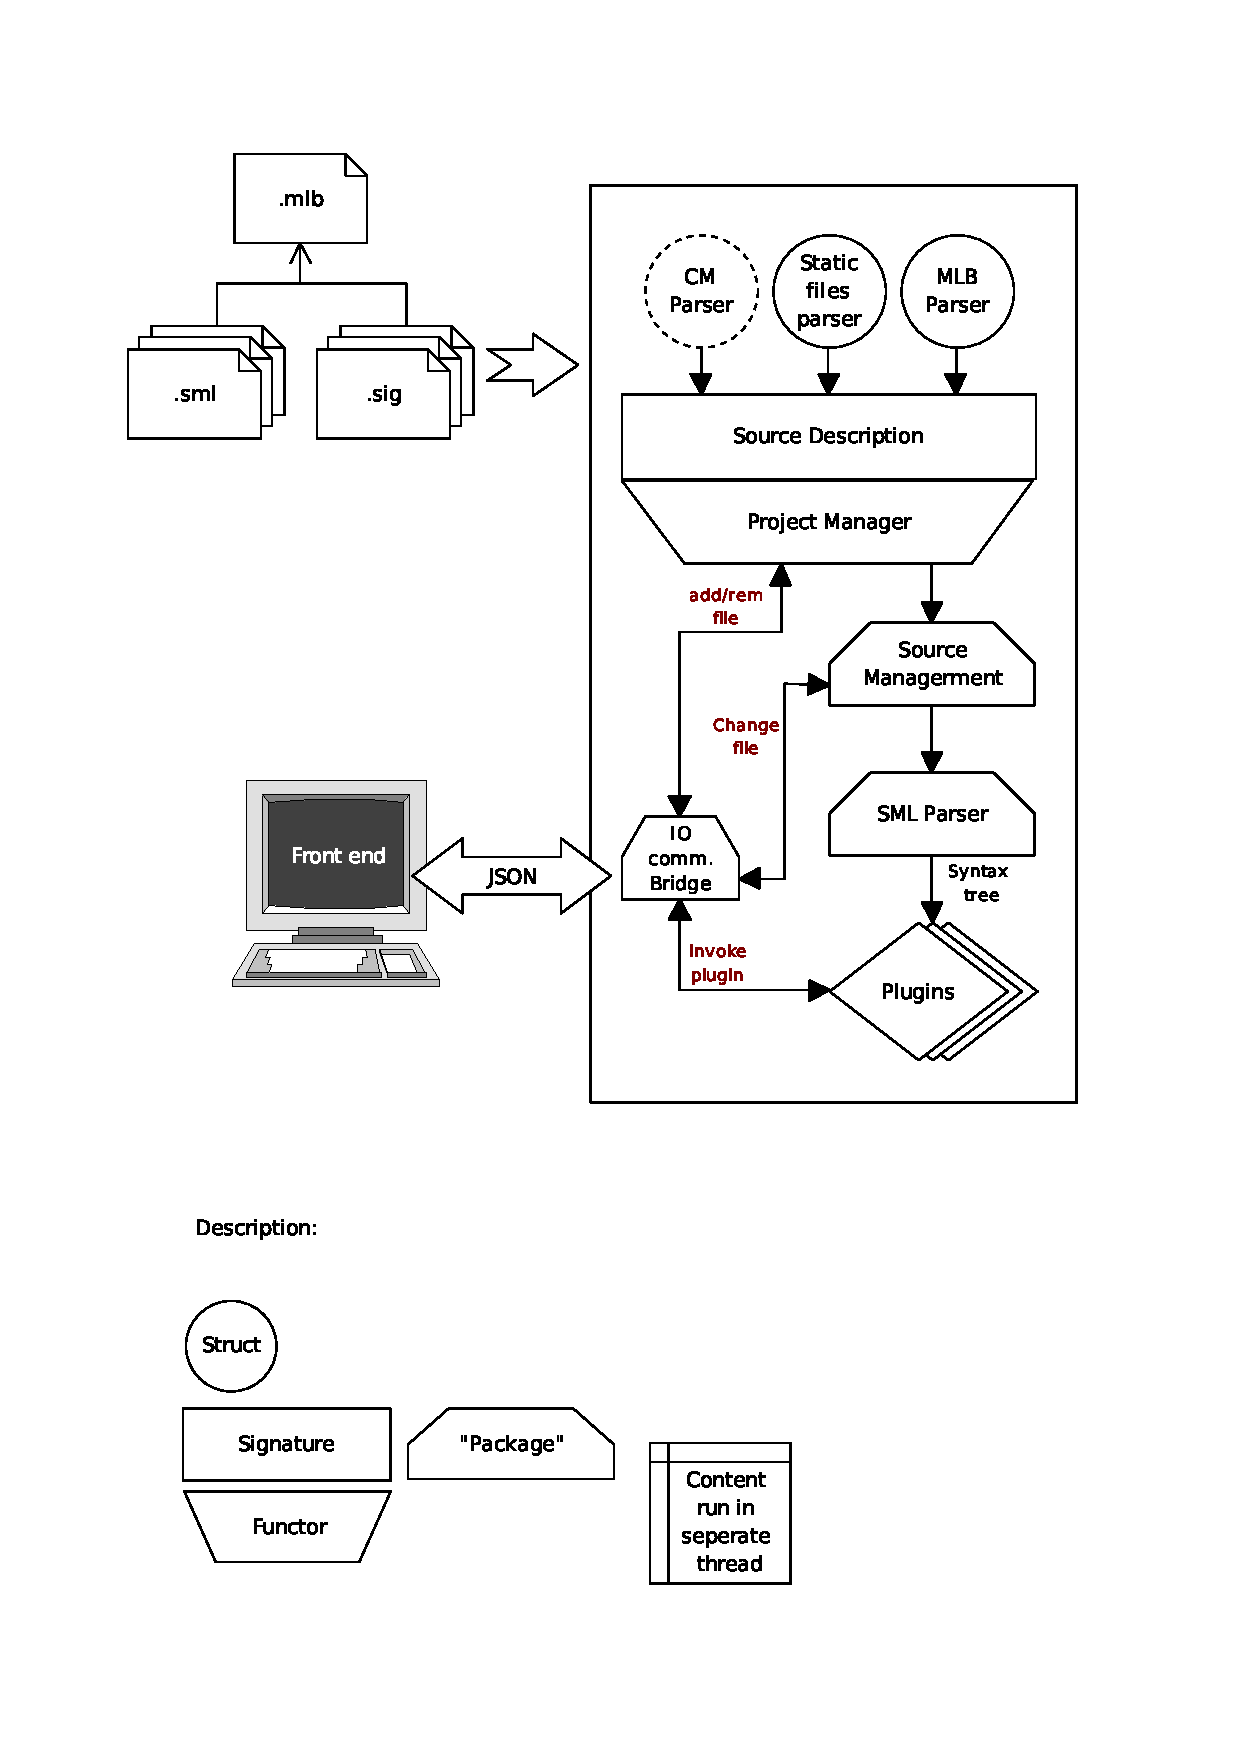
\includegraphics[width=0.9\textwidth]{../drawings/flow}



%\bibliographystyle{plain}
%\bibliography{synopsis}

\end{document}

%%% Local Variables:
%%% mode: latex
%%% TeX-master: t
%%% End:
